Afin de répondre à l'aspect "boîte noire" du modèle utilisé, nous avons im-
plémenté de l'interprétabilité dans notre modèle à l'aide de Grad-CAM~\cite{GRADCAM}.
Cette méthode permet de fournir une explication visuelle vis-à-vis des déci-
sions de classification issue de notre modèle, permettant ainsi de rajouter une
certaine légitimité relative face à nos analyses de traces de sang faisant partie
d'un processus judiciaire. 

L'algorithme Grad-CAM (Gradient-weighted Class Activation Mapping) est une technique utilisée pour rendre les réseaux de neurones convolutifs (CNN) plus interprétables dans le domaine de la classification.
Il fonctionne en générant des cartes de chaleur (heatmaps) qui mettent en évidence les zones importantes d'une image qui contribuent le plus à la prédiction d'une classe spécifique.
Pour ce faire, Grad-CAM calcule les dérivées des scores de sortie de la classe cible par rapport aux caractéristiques de la dernière couche convolutive du CNN.
Ces dérivées sont ensuite globalement moyennées pour obtenir les poids d'importance de chaque carte de caractéristiques.
Enfin, les cartes de caractéristiques sont pondérées par les poids d'importance et combinées pour obtenir la carte de chaleur Grad-CAM, qui peut être superposée à l'image d'origine pour une visualisation plus intuitive.
Cette approche permet de mieux comprendre les décisions prises par le CNN et d'améliorer la confiance dans les prédictions du modèle.

% [exmeple d'une image avec la carte de chaleur Grad-CAM superposée (toute simple pour montrer à quoi ca ressemble)]

\begin{figure}
    \centering
    \begin{subfigure}{0.40\linewidth}
        \centering
        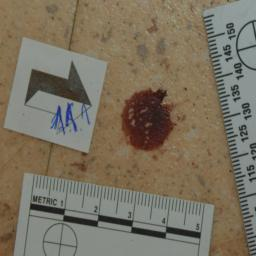
\includegraphics[width=\linewidth]{../asset/exemple/14.jpg}
    \end{subfigure}
    \begin{subfigure}{0.40\linewidth}
        \centering
        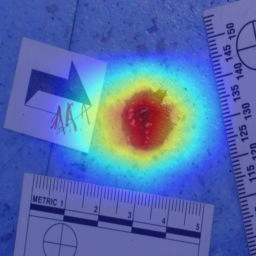
\includegraphics[width=\linewidth]{../asset/exemple/14_saliency.png}
    \end{subfigure}
    \caption{Exemple d'une image  de trace de sang (à gauche) avec sa carte de chaleur Grad CAM superposée (à droite).}
    \label{fig:grad_cam_example}
\end{figure}

Par exemple, nous avons remarqué que parfois certaines des réglettes permettant de donner l'échelle de la photo étaient détectées comme des traces de sang ou induisaient un biais dans la classification.
En utilisant Grad-CAM, nous avons pu identifier que le modèle se focalisait sur ces réglettes pour prendre sa décision, ce qui nous a permis de mieux comprendre
les erreurs de classification et d'améliorer la qualité des prédictions.
% [figure montrant une tache avec une réglette.]
Un autre avantage de Grad-CAM est qu'il permet de vérifier si le modèle se focalise sur la bonne tâche de sang
dans le cas où plusieurs tâches sont présentes sur une même image.

Dans l'exemple suivant, nous voyons que c'est la tâche de gauche qui est détectée par le modèle, ce qui est confirmé par la carte de chaleur Grad-CAM qui met en évidence les zones importantes de l'image pour cette tâche.
% [figure montrant 2 images côte à côte avec les cartes de chaleur Grad-CAM correspondantes].


De plus, nous avons également implémenté la méthode "average drop / average gain /average increase" qui consiste à multiplier l'image de départ par la carte de saillence obtenue avec Grad-CAM puis de redonner cette image au modèle
pour obtenir une nouvelle prédiction.
Cela permet en théorie d'éliminer les parties de l'image qui ne sont pas importantes pour la prédiction et de se focaliser sur les zones importantes, et 
donc d'améliorer la qualité des prédictions du modèle, de renforcer la confiance dans les prédictions et de mieux comprendre les décisions prises par le modèle.

%graphe montrant les 3 équations des 3 méthdoes (3 images cotes a cotes des équations)

% \begin{figure}
%     \centering
%     \begin{minipage}{0.3\textwidth}
%         \centering
%         \includegraphics[width=\textwidth]{../asset/exemple/average_drop.png}
%         \caption{Méthode "average drop".}
%         \label{fig:grad_cam_example1}
%     \end{minipage}\hfill
%     \begin{minipage}{0.3\textwidth}
%         \centering
%         \includegraphics[width=\textwidth]{average_gain.png}
%         \caption{Méthode "average gain".}
%         \label{fig:grad_cam_example2}
%     \end{minipage}\hfill
%     \begin{minipage}{0.3\textwidth}
%         \centering
%         \includegraphics[width=\textwidth]{average_increase.png}
%         \caption{Méthode "average increase".}
%         \label{fig:grad_cam_example2}
%     \end{minipage}
% \end{figure}

Voici les résultats obtenus avec ces méthodes sur une image de trâce de sang:

\begin{table}[h]
    \centering
    \begin{tabular}{lcc}
        \toprule
        Métriques & AWL ResNet & FT AWL ResNet \\
        \midrule
        avg\_drop & 91.6 & 87.6 \\
        avg\_increase & 0.0 & 0.0 \\
        avg\_gain & 0.0 & 0.0 \\
        \bottomrule
        \end{tabular}
    \caption{Résultats des saliency maps sur les données réelles. (Lower is better)}
    \label{tab:saliency_results}
\end{table}
